\documentclass{article}

\linespread{1.5}
\usepackage[utf8]{inputenc}
\usepackage[left=1.35in,right=1.35in,bottom=0.85in]{geometry}
\setlength\parindent{0pt}
\setlength{\parskip}{1em}
\setcounter{secnumdepth}{0}
\usepackage{outlines}
\usepackage{graphicx}
\graphicspath{ {imgs} }
\usepackage[hyphens]{url}
\usepackage{hyperref}
\usepackage{color,soul}
\usepackage[normalem]{ulem}
\usepackage{tabularx}
\usepackage{pgfgantt}
\usepackage[toc]{appendix}
\usepackage{comment}
\usepackage{changepage}
\usepackage{longtable}
\usepackage{tabu}

\usepackage[
backend=biber,
style=apa,
citestyle=authoryear,
sorting=nyt,
]{biblatex}
\addbibresource{refs.bib}

\newcommand{\alignedmarginpar}[1]{%
        \marginpar{\raggedright\small #1}
    }
    
\newcommand{\bisection}[1]{\textbf{\textit{#1}}}

\DeclareCiteCommand{\citeyear}
    {}
    {\bibhyperref{\printdate}}
    {\multicitedelim}
    {}

\title{Research Proposal - Perceived accessibility of urban blue space in Copenhagen}
\author{Carla Hyenne}
\date{}

\begin{document}

\maketitle

\tableofcontents 

%%%%%%%%%%%%%%%%%%%%%%%%%%%%%%%%%%%%%%%%%%%
%				ABSTRACT (500 WORDS)
%%%%%%%%%%%%%%%%%%%%%%%%%%%%%%%%%%%%%%%%%%%
\pagebreak
\section{Abstract}

The benefits of urban nature on people’s health, for fostering community, and for climate change adaptation are widely acknowledged. Within the discourse of environmental justice (EJ), these benefits have been used to demonstrate that equitable access to healthy, unpolluted environments is a human right, with scholars like Anguelovski and Agyeman arguing that marginalised and vulnerable populations are disproportionately affected by lack of access to such spaces. 

Despite extensive studies on the accessibility of urban green spaces (UGS), urban blue spaces (UBS) have not been given the same attention. Moreover, research on UGS accessibility has focused on geographical accessibility, such as proximity to home, and has seldom considered subjective experiences as influencing access. However, accessibility is a multidimensional and complex concept which cannot be reduced to spatial distribution. As Wang, Brown and Liu put forward, perceived accessibility that addresses subjectivities, socio-personal characteristics, and the quality and diversity of the space, must also be considered.

My research addresses the issue of perceived accessibility to UBS by looking at the extent to which subjective experiences and perceptions shape how (un)fairly accessible high-quality, public UBS interventions are, and what this means for the environmentally just city.
I will pay special attention to socio-economic and personal characteristics such as age, gender, income, ethnicity, cultural practices, and general preferences for infrastructure and aesthetics.

Specifically, I will be looking at three blue spaces in Copenhagen located in neighbourhoods with varying socio-economic and demographic profiles. A combination of observations of human activity and site quality, and surveys with users, will allow me to study a variety of perspectives on UBS. I will discuss the extent to which the city of Copenhagen offers equitable opportunities for people with different backgrounds and preferences to enjoy UBS, and juxtapose this against the ideal of the environmentally just city. 
Given the availability of UBS in Copenhagen and the importance the city is giving to harbour baths and urban beaches, it will be particularly useful to evaluate whether Copenhagen’s UBS caters to everyone’s needs.

I argue that perceived accessibility is an important dimension of EJ, because public UBS are places of community, attachment, and well-being. Ignoring subjective experiences that differ from the mainstream can contribute to social inequalities, discrimination, and displacement.

In conclusion, my research will closely examine how perceptions shape accessibility to UBS. It will serve to understand what perceptions and experiences those who control access (city planners) must take into account if UBS are to be usable by everyone.

%%%%%%%%%%%%%%%%%%%%%%%%%%%%%%%%%%%%%%%%%%%%
%								LITERATURE REVIEW (2-3 PAGES)
%%%%%%%%%%%%%%%%%%%%%%%%%%%%%%%%%%%%%%%%%%%%
% INTRO
% Blue spaces definition: natural and semi-natural areas
\pagebreak
\section{Literature review}

This section reviews the academic literature on urban blue spaces (UBS). It introduces concepts that are central for understanding the use of UBS, namely ecosystem services, environmental justice and social barriers. Although a lot of the literature mentioned is focused on green spaces, the similarities between green and blue spaces with regards to social and environmental effects give grounds for judiciously extending the research to include blue spaces. Moreover, many blue spaces have some green space and vice versa.

%%%%%%%%%%%%%%%%%%%%
\subsection{The benefits of urban blue space}
%%%%%%%%%%%%%%%%%%%%

%%% Ecosystem system services as a way to understand the value that people, and cities as a whole, can derive from urban nature
%In an urban context, UBS has undeniable positive effects on people and the environment, which Gascon et al. (\citeyear{gascon2017outdoor}) summarise as ``stress reduction, increased physical activity, promotion of positive social contacts, increased place attachment and the reduction of extreme temperatures''. These benefits can be understood under the broad categories of health and ecosystem services. Within ecosystem services, we distinguish two realms, namely cultural and regulating.

UBS are a network of natural or semi-natural areas dominated by water, and designed to provide a range of ecosystem services, which themselves provide social and environmental benefits.

%%% Cultural ES
Firstly, cultural ecosystem services refer to the intangible benefits that people derive from their relationship to nature. These benefits include recreation and well-being, cultural and spiritual practices, opportunities for education, or community forming and belonging \parencite{phillips2021use}. A recent example of people discovering the cultural value of urban blue and green spaces is the COVID-19 pandemic. During the strict lockdown measures implemented by governments worldwide, people (re)discovered the value of parks, forests, rivers and lakes as places to escape from home and interact safely with others in an open space \parencite{kohsaka2021urban}. 
% IS THIS CULTURAL ES?
UBS also provide physical and mental health benefits - being exposed to water makes people feel better and happier. There is an extensive repertoire of quantitative studies demonstrating these effects on people's health and well-being (\cite{gascon2017outdoor}, \cite{britton2020blue}), and qualitative studies also show that exposure to UBS improves mental health, regardless of how people interact with it (\cite{garrett2019urban}, \cite{van2021urban}).

%%% Regulating ES for climate extremes
Secondly, regulating ecosystem services refer to the power that nature has to mitigate extreme events, particularly in relation to climate change. When blue and green infrastructure work in tandem, they can alleviate heat stress by acting as cooling islands (\cite{gunawardena2017utilising}, \cite{lin2020water}) or provide protection from heavy rainfall and flooding through the design of natural stormwater management systems like flood plains (\cite{o2020sustainable}, \cite{ghofrani2017comprehensive}). Moreoever, water is necessary for  any green infrastructure to sustain itself and provide well-known benefits like reducing air pollution \parencite{pugh2012effectiveness}. Thus, when planned in accordance with local environmental features, blue-green infrastructure can increase the climate resiliency of cities \parencite{o2021international}.

% TODO --> Lastly, ecosystem services can be multifunctional such that one UBS can fulfill more than one ecosystem service \parencite{plieninger2022disentangling}.

%%% Thesis --> benefits of UBS for biodiversity. Ref \parencite{kimic2021assessment} on biodiversity (1.2.2)

Given the potential benefits of UBS on people and the environment, providing public UBSs that meet the needs of residents contributes to creating socially and environmentally resilient cities.
 
%%%%%%%%%%%%%%%%%%%%
\subsection{The renewal of urban blue space}
%%%%%%%%%%%%%%%%%%%%

%Most large cities are located near water, either inland like rivers, lakes or harbours, or on the coast. 
With urbanisation, rivers, lakes and harbours in cities were polluted or transformed by industries \parencite{kampa_langaas_anzaldua_2016}, and became unattractive and unsafe to swim in.
In the 20th century, post-industrial European cities started considering UBSs as strategic opportunities to revitalise the city \parencite{del2021dismantling}. Over the last few decades, the importance of UBS has entered public consciousness in part due to climate concerns.
Through local and international political pressure and public demand, governments invested in the renewal of UBSs into attractive places for people to use. % TODO REF

\subsubsection{Positive effects of urban blue space renewal}

%%% Ways in which UBS renewal is positive: building community; cleaning up polluted spaces;
In addition to the aforementioned cultural ecosystem services, UBS renewal projects can provide specific social benefits like community building. They are an opportunity to engage residents in the design and implementation process. In a deprived area of Plymouth, in the UK, a small-scale UBS intervention revealed that residents who participated in the project reported a greater sense of well-being and life satisfaction due to feelings of community belonging and an increased sense of safety in their neighbourhood \parencite{van2021urban}.

%%% TODO something more about ubs renewal benefits??
%%% Bring in EJ? as a principle which illustrates the need to provide safe, clean, unpolluted environments for all

%%%%%%%%%%%%%%%%%%%%
\subsubsection{Social consequences of urban blue space renewal}
%%%%%%%%%%%%%%%%%%%%
% thesis --> add ``and the environment'' and clarify how improvements to UBS can harm environment

Despite the undeniable benefits of water in the city, upgrading UBSs into clean and attractive public spaces can have undesirable social consequences.
Two mechanisms of action are exclusionary planning and the effect on the real estate market.
% \sout{These reinforce socio-spatial inequalities by discriminating against people on the basis of socio-economic and cultural differences, or by way of racist and sexist practices.}

%%% Exclusionary planning can disrupt local communities
First, in contrast to the social bonds that can be fostered when residents are involved in renewal projects, UBS interventions can disrupt connections between people and with nature.
This is exacerbated by the tendency to view polluted or degraded UBS as having less value than clean and attractive spaces \hl{REF}. 
But Toomey et al. (\citeyear{toomey2021place}) demonstrate in their research on Coney Island Creek, in New York City, that people can attach meaning to degraded UBS. Despite the water being heavily polluted, the Creek supports a range of activities and social connections, and there are concerns from local experts that future renewal may disrupt these practices. One way to overcome this is for planners to consult local communities during the design and implementation of any UBS project.

However, marginalised or stigmatised communities may find it hard to communicate their experience when consulted by planners, because they lack a common language to articulate their reality. And vice-versa: wealthy, white, males may not be capable of understanding the experience of `others' \parencite{anguelovski2020expanding}. To this end, Toomey et al. (idib.) propose using language like ``place-disruption'' and ``place-protection'' to promote mutual understanding and avoid privileging the values of mainstream groups over those of marginalised communities.

%%% Effects of UBS renewal on the housing market/`green' gentrification
Second, local governments are using UBS to brand their cities as `green' and liveable. Two examples are the Madrid Río project advertised on Madrid's official tourism website, as ``ideal to cool down'' and with infrastructure ``made from sustainable, natural materials'' \parencite{madridrio}; and Oslo advertising its urban waterfront promenade along which you can admire the city's starchitecture \parencite{visitoslo}.

Cities are also using greening - the process of upgrading urban settings into environmentally more sustainable spaces - as a win-win strategy where ``no one is left behind by the trickle-down of benefits from green infrastructure'' \parencite{anguelovski2021green}. However, there is a mismatch between cities trying to attract new creative classes through UBS renewal, and with addressing UBS as a common good and prioritising the concerns of existing residents (\cite{wessells2014urban}, \cite{anguelovski2020expanding}).
These strategies can perpetuate inequalities by privileging the values of white, environmentally privileged upper classes who can afford to live near nature \parencite{anguelovski2021green}. This phenomenon is referred to as green gentrification, where greening can contribute to the exclusion and displacement of residents who are priced out of the housing and rental markets and must move to a neighbourhood with less attractive nature.

%%%%%%%%%%%%%%%%%%%%
\subsection{The environmental justice principle}
%%%%%%%%%%%%%%%%%%%%

To articulate the phenomenon by which UBSs provide social and environmental benefits, but at the same time discriminate against vulnerable populations, scholars have used the concept of environmental justice.
Starting as a social movement in the 1980s, environmental justice puts forward the principle that everyone should have equal opportunities to access clean, healthy, unpolluted spaces. It has since concretised into an academic discourse that looks at a range of factors affecting the opportunities people have to access urban nature. 

% perceptions address all of recognition, procedural, and distributive justice (ref plieninger)

% ej looks at, eg. the location of UBS in the city, discrimination in public participation and decision making with regards to UBS renewal, and individual and community perceptions and preferences which may influence how people interact, or not, with the space.

%The applications of EJ on UBS are limited in comparison to urban green space. One study that stands out is Raymond et al.'s (\citeyear{raymond2016integrating}) research on the diversity of people, activities and perceived unpleasant experiences in Helsinki's blue spaces. The wide range of opinions they find show the importance of considering a multitude of perceptions when planning UBS, because people of different age, income, gender, ethnicity, etc. have varying preferences.

%%%%%%%%%%%%%%%%%%%%
\subsection{Barriers to using urban blue space}
%%%%%%%%%%%%%%%%%%%%

% barriers to `realising' the benefits of UBS

Barriers are understood as anything that prevents people from using, or feeling like they can use, UBS.
These barriers can be physical, or non-physical (\cite{biernacka2018classification}, \cite{wolff2022conceptualizing}. Physical barriers can be the existence of UBS in the city, their distribution, accessibility by different modes of transit, or distance from home. Non-physical barriers, are personal factors refering to social, economic or cultural aspects that affect perceptions and preferences in the built environment and social setting, or feelings of safety or belonging. These barriers are influenced by institutional context, ie. the ``formal and informal rules of a governance system that shapes human choices, behaviours and interactions'' \parencite{wolff2022conceptualizing}. Institutions set the societal norms, and are influenced by individuals as well as local and national governments and organisations.

To analyse the use of green space, Biernacka and Kronenberg (\citeyear{biernacka2018classification}) propose looking at availability, accessibility and attractiveness (a version of this framework is summarised in figure ~\ref{fig:diagram_ubs_use}).
Availability refers to the physical presence of green space, and accessibility to the physical and perceived reachability of the space - whether it can be reached in reasonable time, or seen as open and public (not private). 
They argue that the first two, availability and accessibility, must be fulfilled before people can evaluate attractiveness and consider using the space. It follows that an abundance of UBS does not necessarily mean that demand is met, if individual needs are not satisfied \parencite{phillips2021use}.

\begin{figure}[ht]
	\makebox[\textwidth][c]{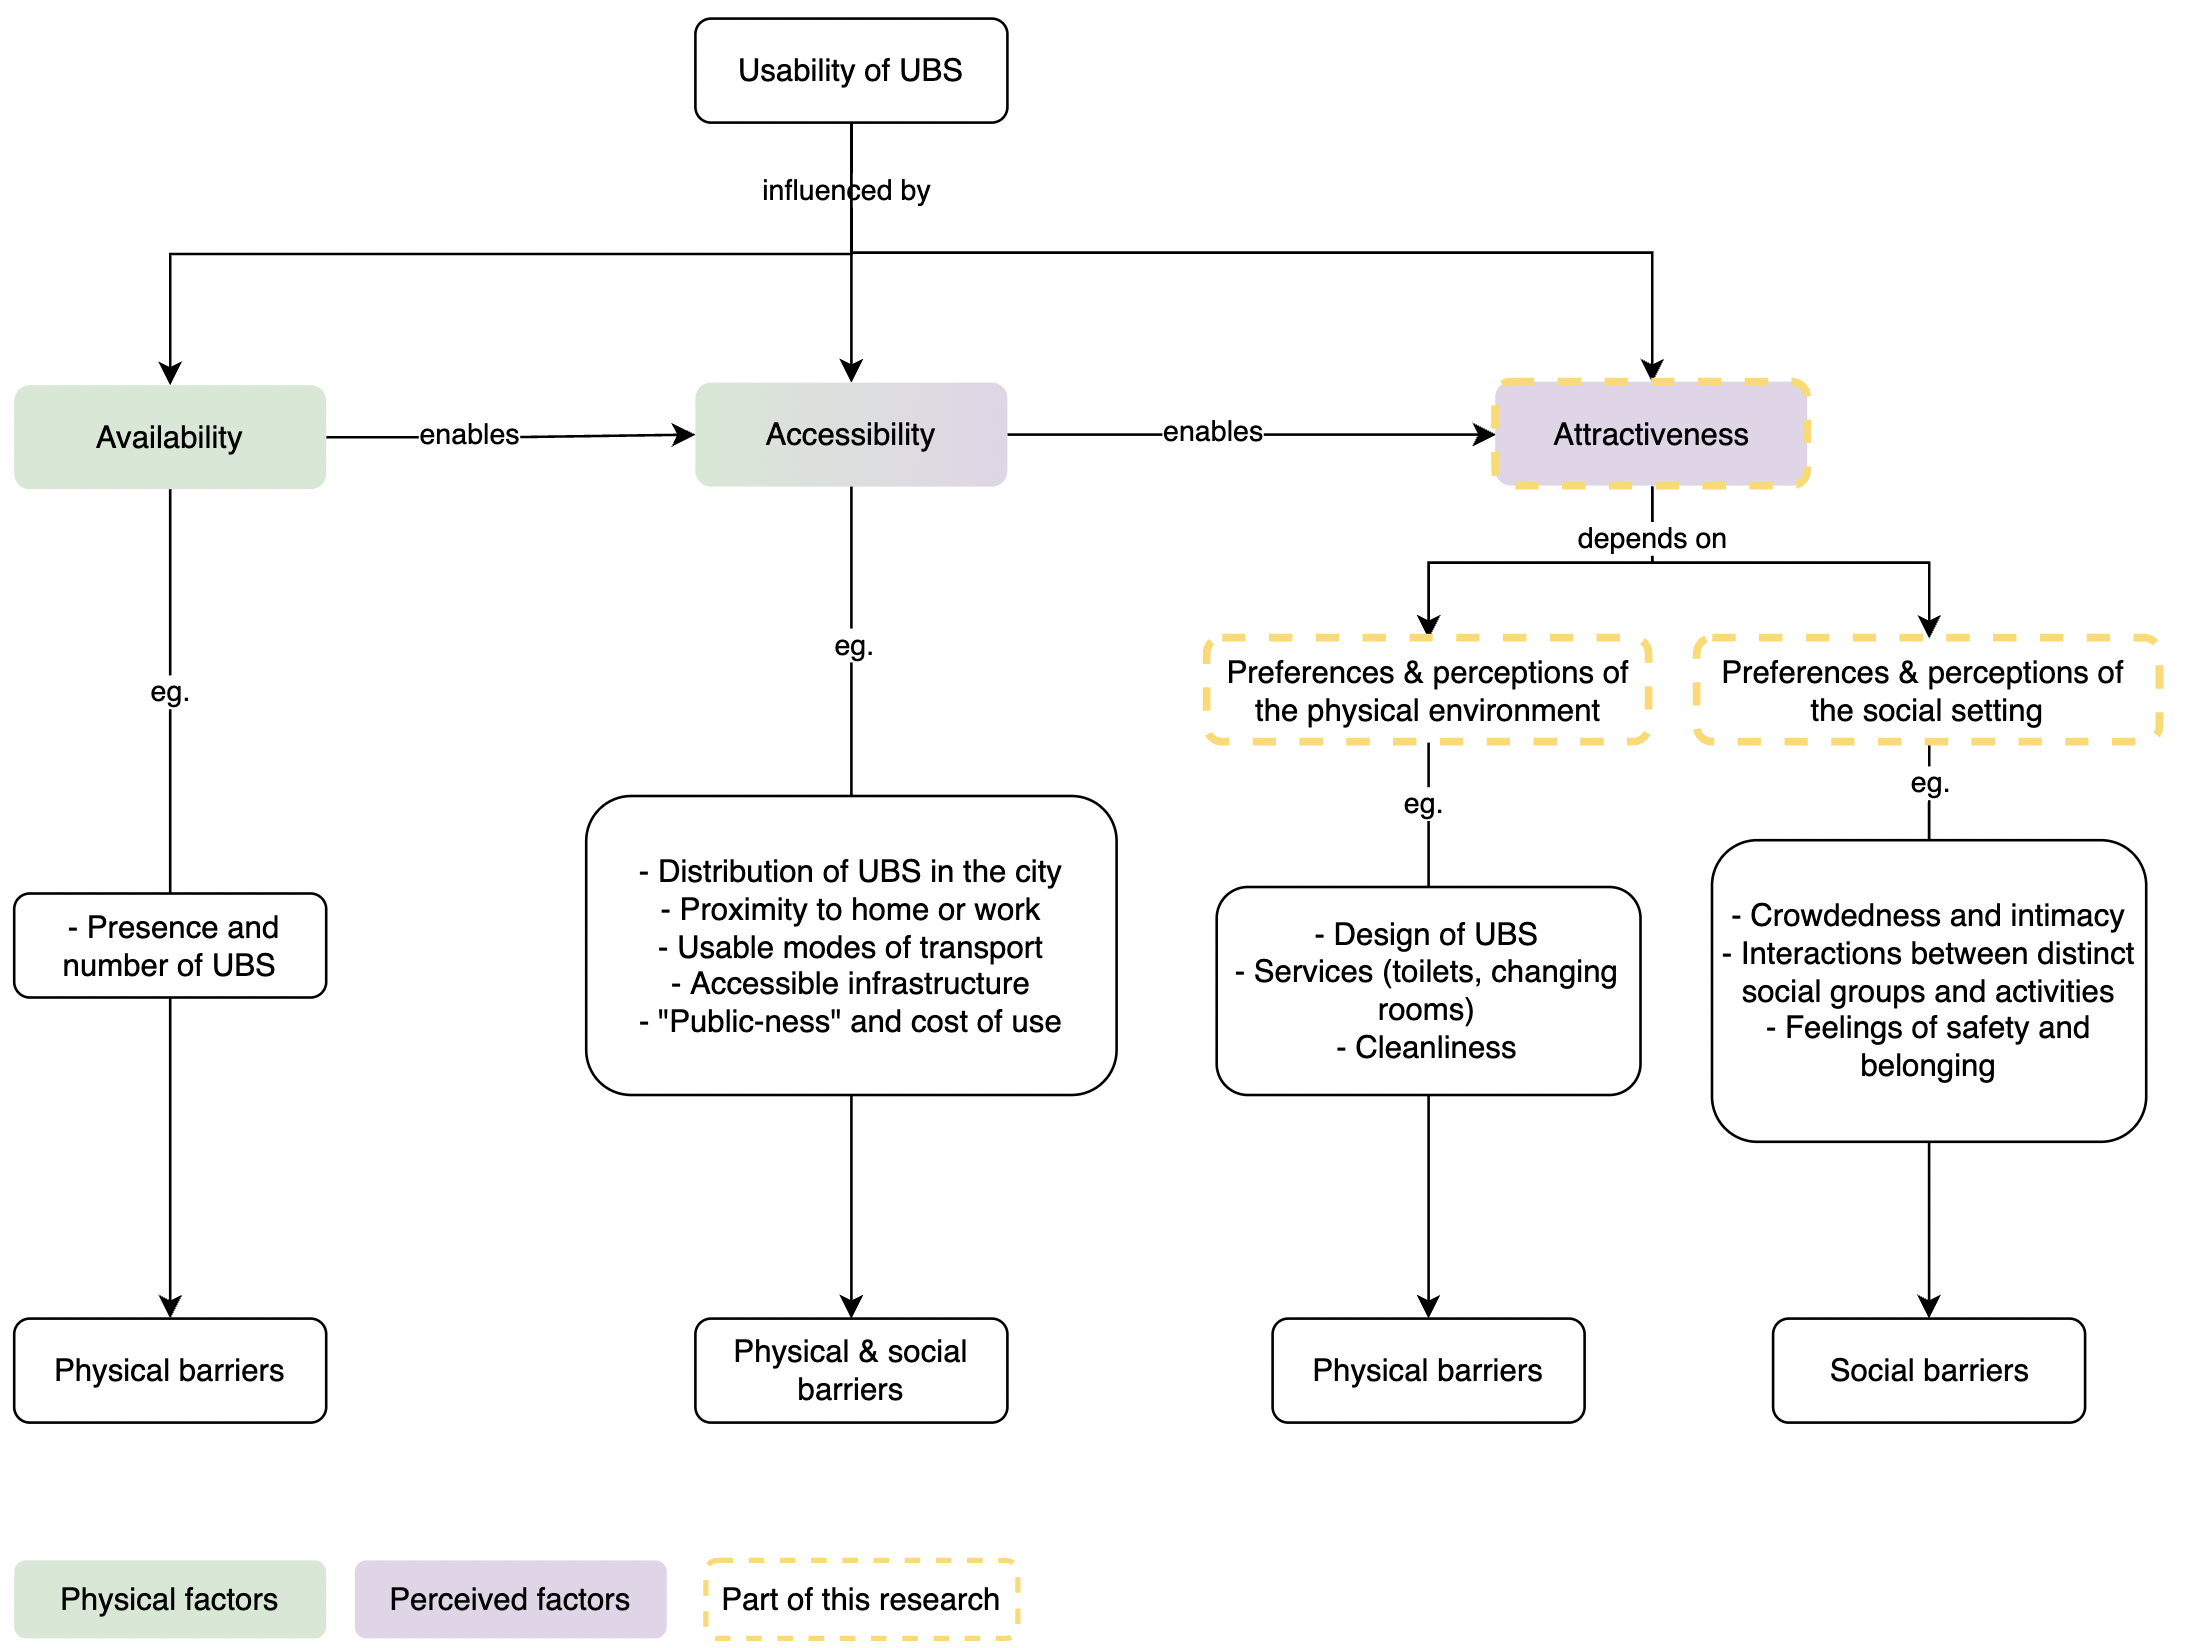
\includegraphics[width=1.2\textwidth]{diagram_ubs_use.png}}
	\caption{\textit{A diagram summarising the three factors influencing usability of UBS according to Biernacka and Kronenberg (\citeyear{biernacka2018classification}), namely availability, accessibility and attractiveness, along with examples of physical and social barriers that influence the fulfillment of these factors.}}
	  \label{fig:diagram_ubs_use}
\end{figure}

There are a variety of factors that go into deciding whether or not a space is attractive. For example in their research, Phillips et al. (ibid.) analyse people's motivations and preferences for using certain green spaces in Brussels. They find that there are two distinct groups of people: those who use parks to be close to nature, and those who go to parks to be surrounded by people.
These different expectations illustrate the need for renewal projects to consider social and personal nuances that go beyond presence and reachability of UBS.

To date, studies that evaluate the degree to which people can make use of urban nature have focused not only on green spaces, but also on measuring geographical factors like availability and physical accessibility (\hl{REFs}).
But as I have mentioned, the reasons for using green spaces or UBS are complex and multidimensional, and cannot be reduced to a purely physical aspect \parencite{wang2015physical}. Perceived barriers stemming from subjective experiences are equally as important.

From the perspective of environmental justice, it is important to consider perceptions in explaining the mismatch between provision and use of UBS because variations in socio-economic status (age, gender, ethnicity, education, income, etc.) influence how people perceive UBS and its potential benefits (\cite{plieninger2022disentangling}, \cite{phillips2021use}). In neighbourhoods with lower socio-economic status, the use of green space is often lower than in more affluent neighbourhoods, despite similar opportunities to access green spaces (\cite{wang2015comparison}, \hl{REF}). As such, perceptions can lead to unequal opportunities to access clean and healthy green, or blue, spaces.

% What are perceived barriers vs. social barriers??ref \parencite{noel2021social}.???
% can be explained by a range of perceived barriers preventing people from finding the space attractive ref \parencite{noel2021social}.

%%% TODO --> todo read Cronin-de-Chavez et al.

%%%%%%%%%%%%%%%%%%%%%%%%%%%%%%%%%%%%%%%%%%%%%%
%								PROBLEM STATEMENT AND RQ (1 PAGE)
%%%%%%%%%%%%%%%%%%%%%%%%%%%%%%%%%%%%%%%%%%%%%%

\section{Problem Statement}

% Ideal
The principle of environmental justice entails equitable access to healthy, unpolluted environments, such as clean, public UBS. This is important because water in the city provides cultural and regulating ecosystem services.
% Real
In reality, a multitude of physical and perceived barriers exist which may prevent individuals or communities from visiting UBS, even if they live nearby. And while there is considerable research on the physical barriers, and to some extent social barriers, to green space, studies focusing on UBS are limited.
% Consequences
However, UBS share similar social and environmental benefits to green spaces, and natural bodies like rivers and lakes are relatively immobile. This means that they cannot be planned in the same way as public parks, and that perceived and social factors may be more relevant than geographical elements to understand use patterns.

Understanding this phenomenon is important because public UBS are places of community, identity, attachment, and well-being. Ignoring subjective experiences with regards to UBS can exclude relevant actors from planning processes, and ultimately produce unfair outcomes \parencite{plieninger2022disentangling}. 
As such, it is worthwhile to explore the perceptions of UBS users, to understand what social, personal or economic factors enable or inhibit them from visiting different UBS in the city, in order to design more effective policies and planning strategies to increase the use of UBS for everyone.

% Research question
Given the above, my research aims to answer the following question: \textbf{how do perceptions and subjective experiences shape how (un)fairly usable public blue space interventions are, and what does this mean for the environmentally just city?}

%%%%%%%%%%%%%%%%%%%%%%%%%%%%%%%%%%%%%%%%%%%%%%
%							RESEARCH DESIGN (4-6 PAGES)
%%%%%%%%%%%%%%%%%%%%%%%%%%%%%%%%%%%%%%%%%%%%%%
\section{Methodology}

%\sout{My research will be explanatory because I aim to explain whether or not there are equal opportunities for people to access UBS. I will take an inductive approach, whereby my theory will emerge from the data I will collect on people’s uses and perceptions of UBS, and on the quality and diversity of the sites. The theories framing the research are environmental justice - everyone should have equal access clean, unpolluted, healthy environments - and perceived accessibility - the subjective, socio-personal, preferential characteristics that shape access}

%%%%%%%%%%%%%%%%%%%%
\subsection{Case study}
%%%%%%%%%%%%%%%%%%%%

The research will compare perceived barriers to UBS in three different UBS in the city of Copenhagen, which makes for an interesting case for the following four reasons. First, Copenhagen is located on the Kattegat strait, has a high availability of UBS with 92 km of coastline, and water features prominently in the urban landscape \parencite{comertler2017greens}. Second, the city trying to position itself as a world leader in sustainability and is doing so by making its shoreline attractive. Since 2002, there have been over ten blue space rehabilitation projects in the form of harbour baths and urban beaches, which are now open to the public and free to use \parencite{visitcopenhagen_baths}. Third, Copenhagen is experiencing an increase in poverty and ethnic segregation \parencite{moller2015socioeconomic}, as well as a growing racist discourse in the media and politics. For example, through the classification of some neighbourhoods as ‘ghettos’ \parencite{simonsen2008practice}. This evolving socio-economic landscape and its surrounding discourse make it important to understand who feels like they can access UBS, and who might not. Finally, Copenhagen’s reputation as one of ``the most liveable cities'' \parencite{visitdenmark_2021}, due in part to the swimming spots in the harbour, begs the question - for whom is the city liveable, if not all can use the UBS?

% TODO map distance of UBS to place of residence/400m from building blocks

\subsubsection{Potential cases}

Every UBS and neighbourhood has a different set of social, economic, political, cultural or environmental conditions which influence who uses it, why, and how they feel in it. In order to uncover these conditions, the units of analysis should be scoped to specific locations on the waterfront, and match three criteria:

\begin{enumerate}
	\item The UBS should allow people to carry out a multitude of activities like sitting, swimming, socialising, playing sports, etc. to ensure people have the opportunity to carry out their prefered activities
	\item The sites should have been renewed by the city, be public and free to use so there are no monetary barriers
	\item The UBSs should be located in neighbourhoods with distinct socio-economic profiles, since perceptions are rooted in socio-economic, cultural and personal factors
\end{enumerate}

The maps in figure \ref{fig:map_income} represent income and education statistics of districts in Copenhagen, retrieved from Denmark's statistic bank \parencite{copenhagenStatbank}. These statistics, along with the list of harbour baths and beaches on the VisitCopenhagen website \parencite{visitcopenhagen_baths}, served to shortlist five UBS: the Sandkaj harbour bath, the Svanemøle beach, the Sluseholmen harbour bath, the Amager beach and the Kastrup sea bath (see Figure \ref{fig:ubs}). I will not be able to study five UBSs, but a more detailed neighbourhood analysis and a visit to the spaces is required to make a final decision. 

I also considered inland UBS such as lakes or rivers, which would be interesting to compare with the high-profile harbours and beaches. However I could not identify any that supported many activity (ie., it was not possible to swim, play sports, sit, etc.). Visiting these spaces in person might change my interpretation.

\begin{figure}[ht]
	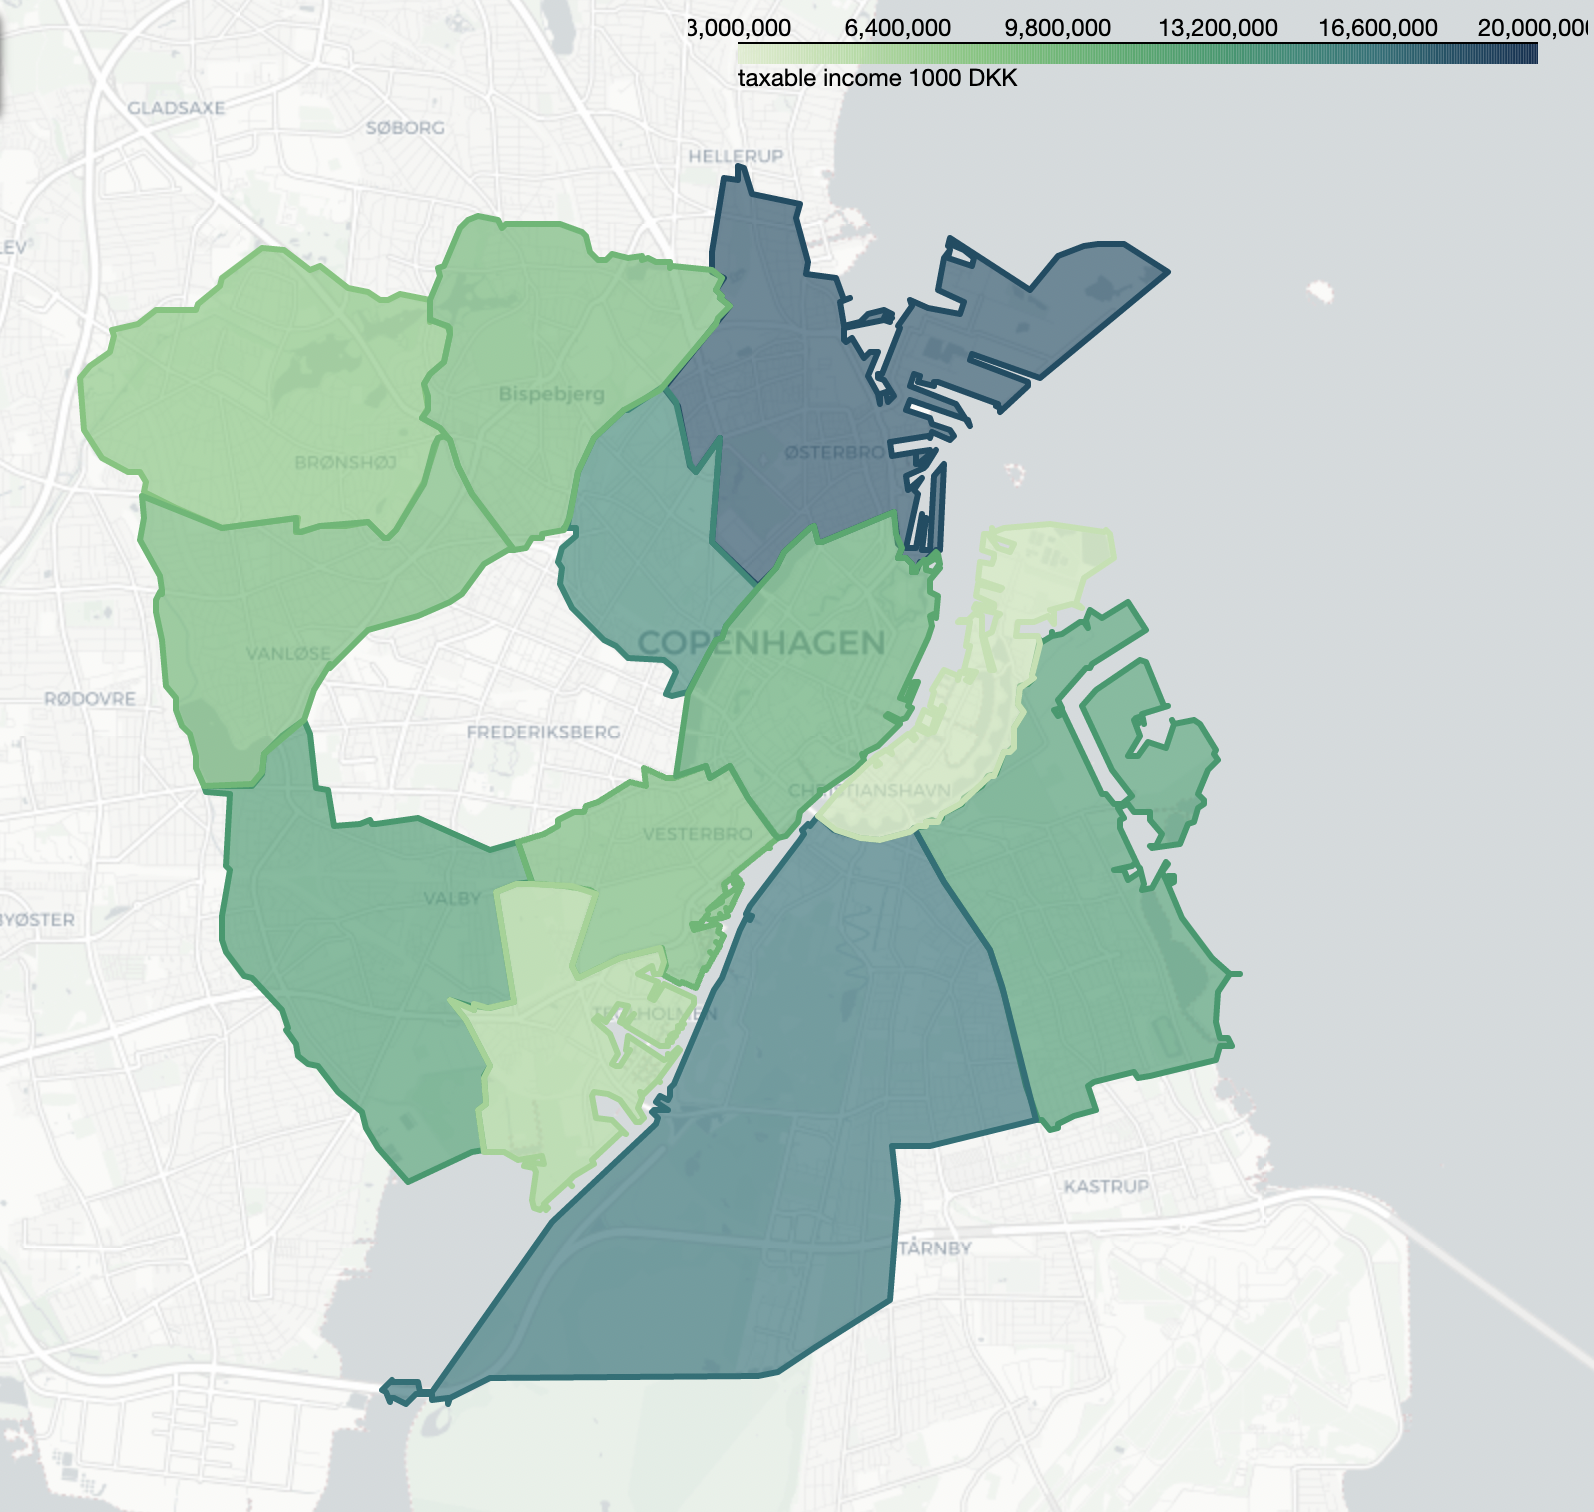
\includegraphics[width=0.5\textwidth]{copenhagen_income_taxable.png}
	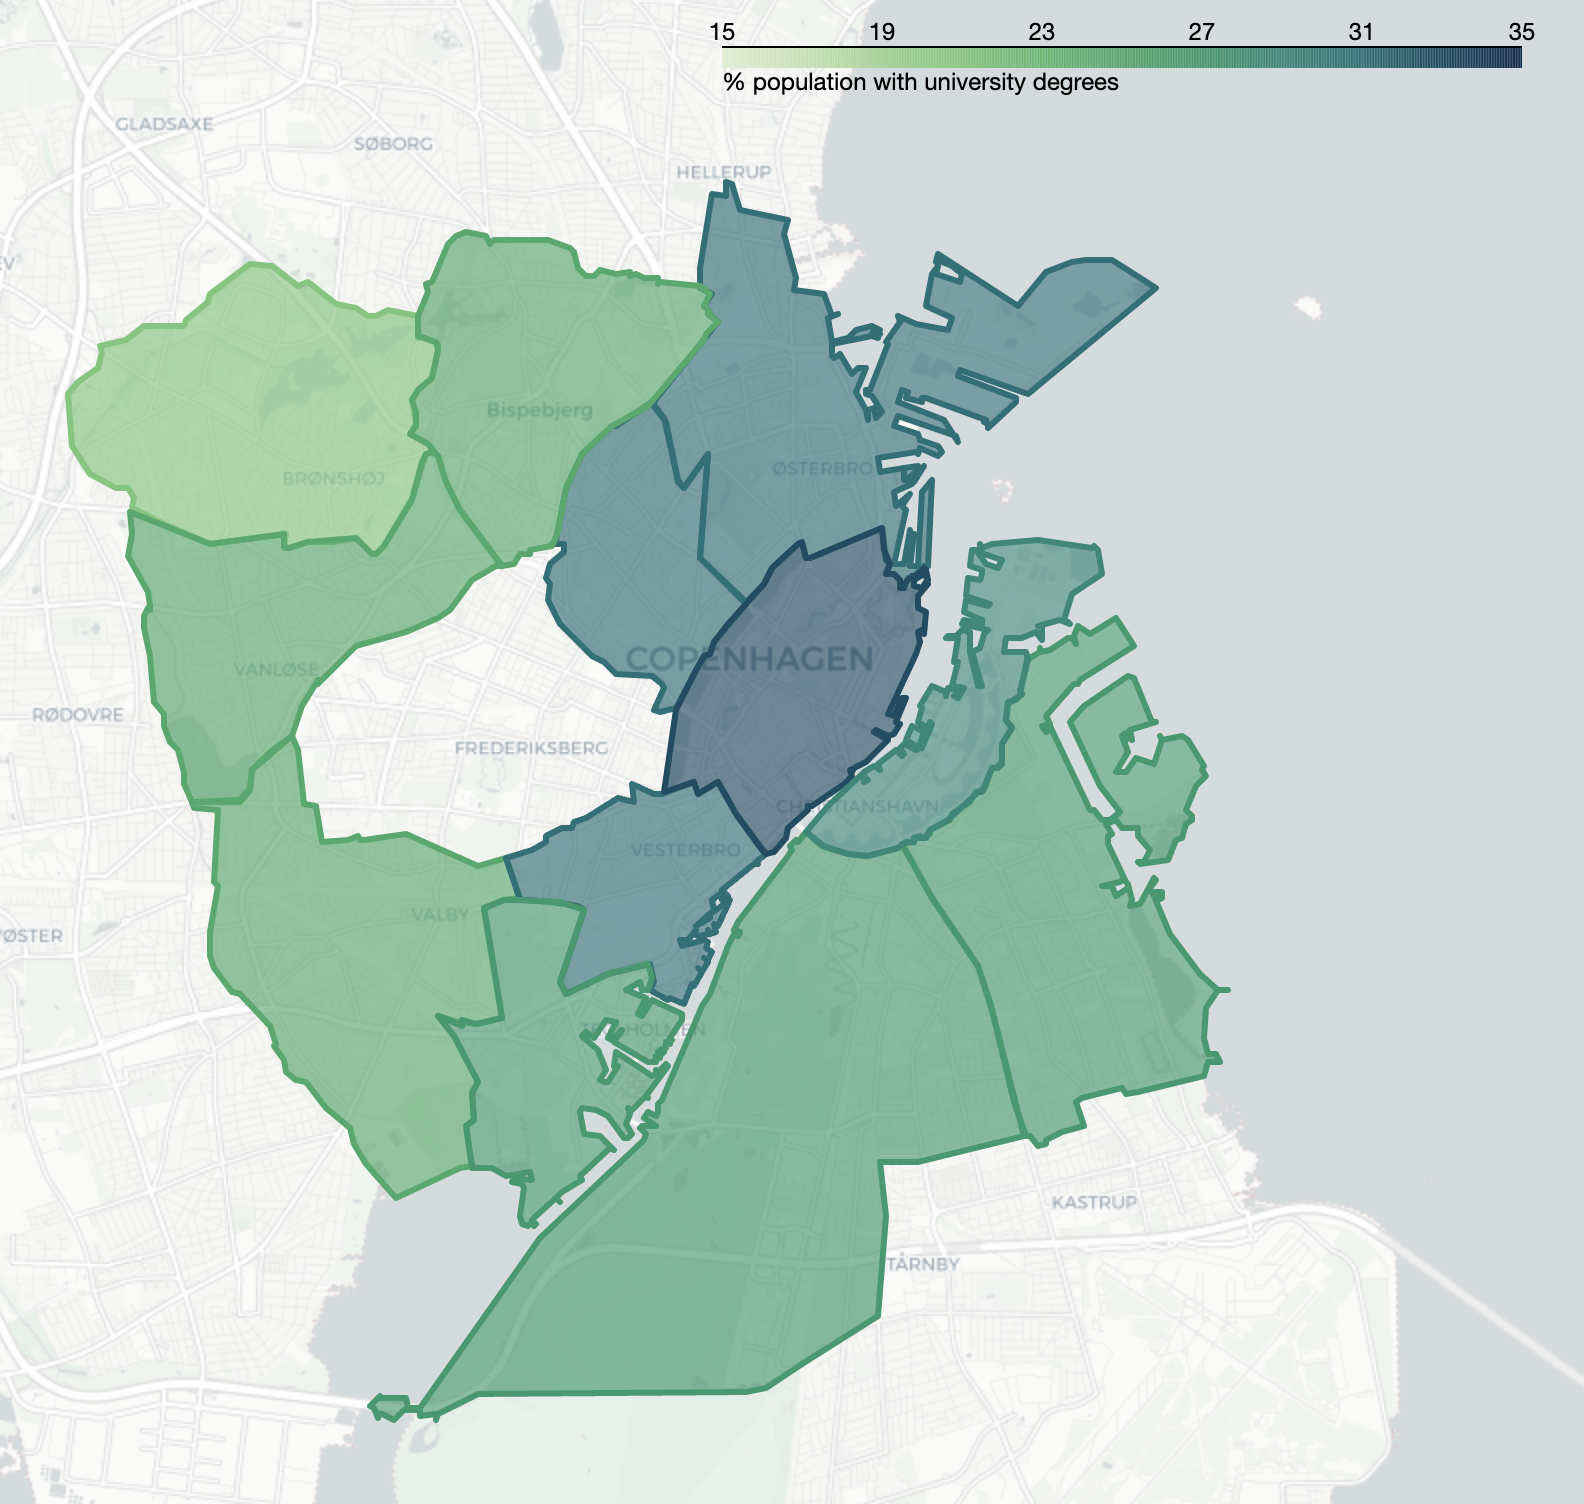
\includegraphics[width=0.5\textwidth]{copenhagen_edu.png}
	\caption{\textit{Left: taxable income (in 1000 DKK) the districts of Copenhagen for the year 2020. Right: percentage of residents with a university degree (Bachelor, Master or PhD) in the districts of Copenhagen for the year 2020.}}
	  \label{fig:map_income}
\end{figure}

\begin{figure}[ht]
	\centering
	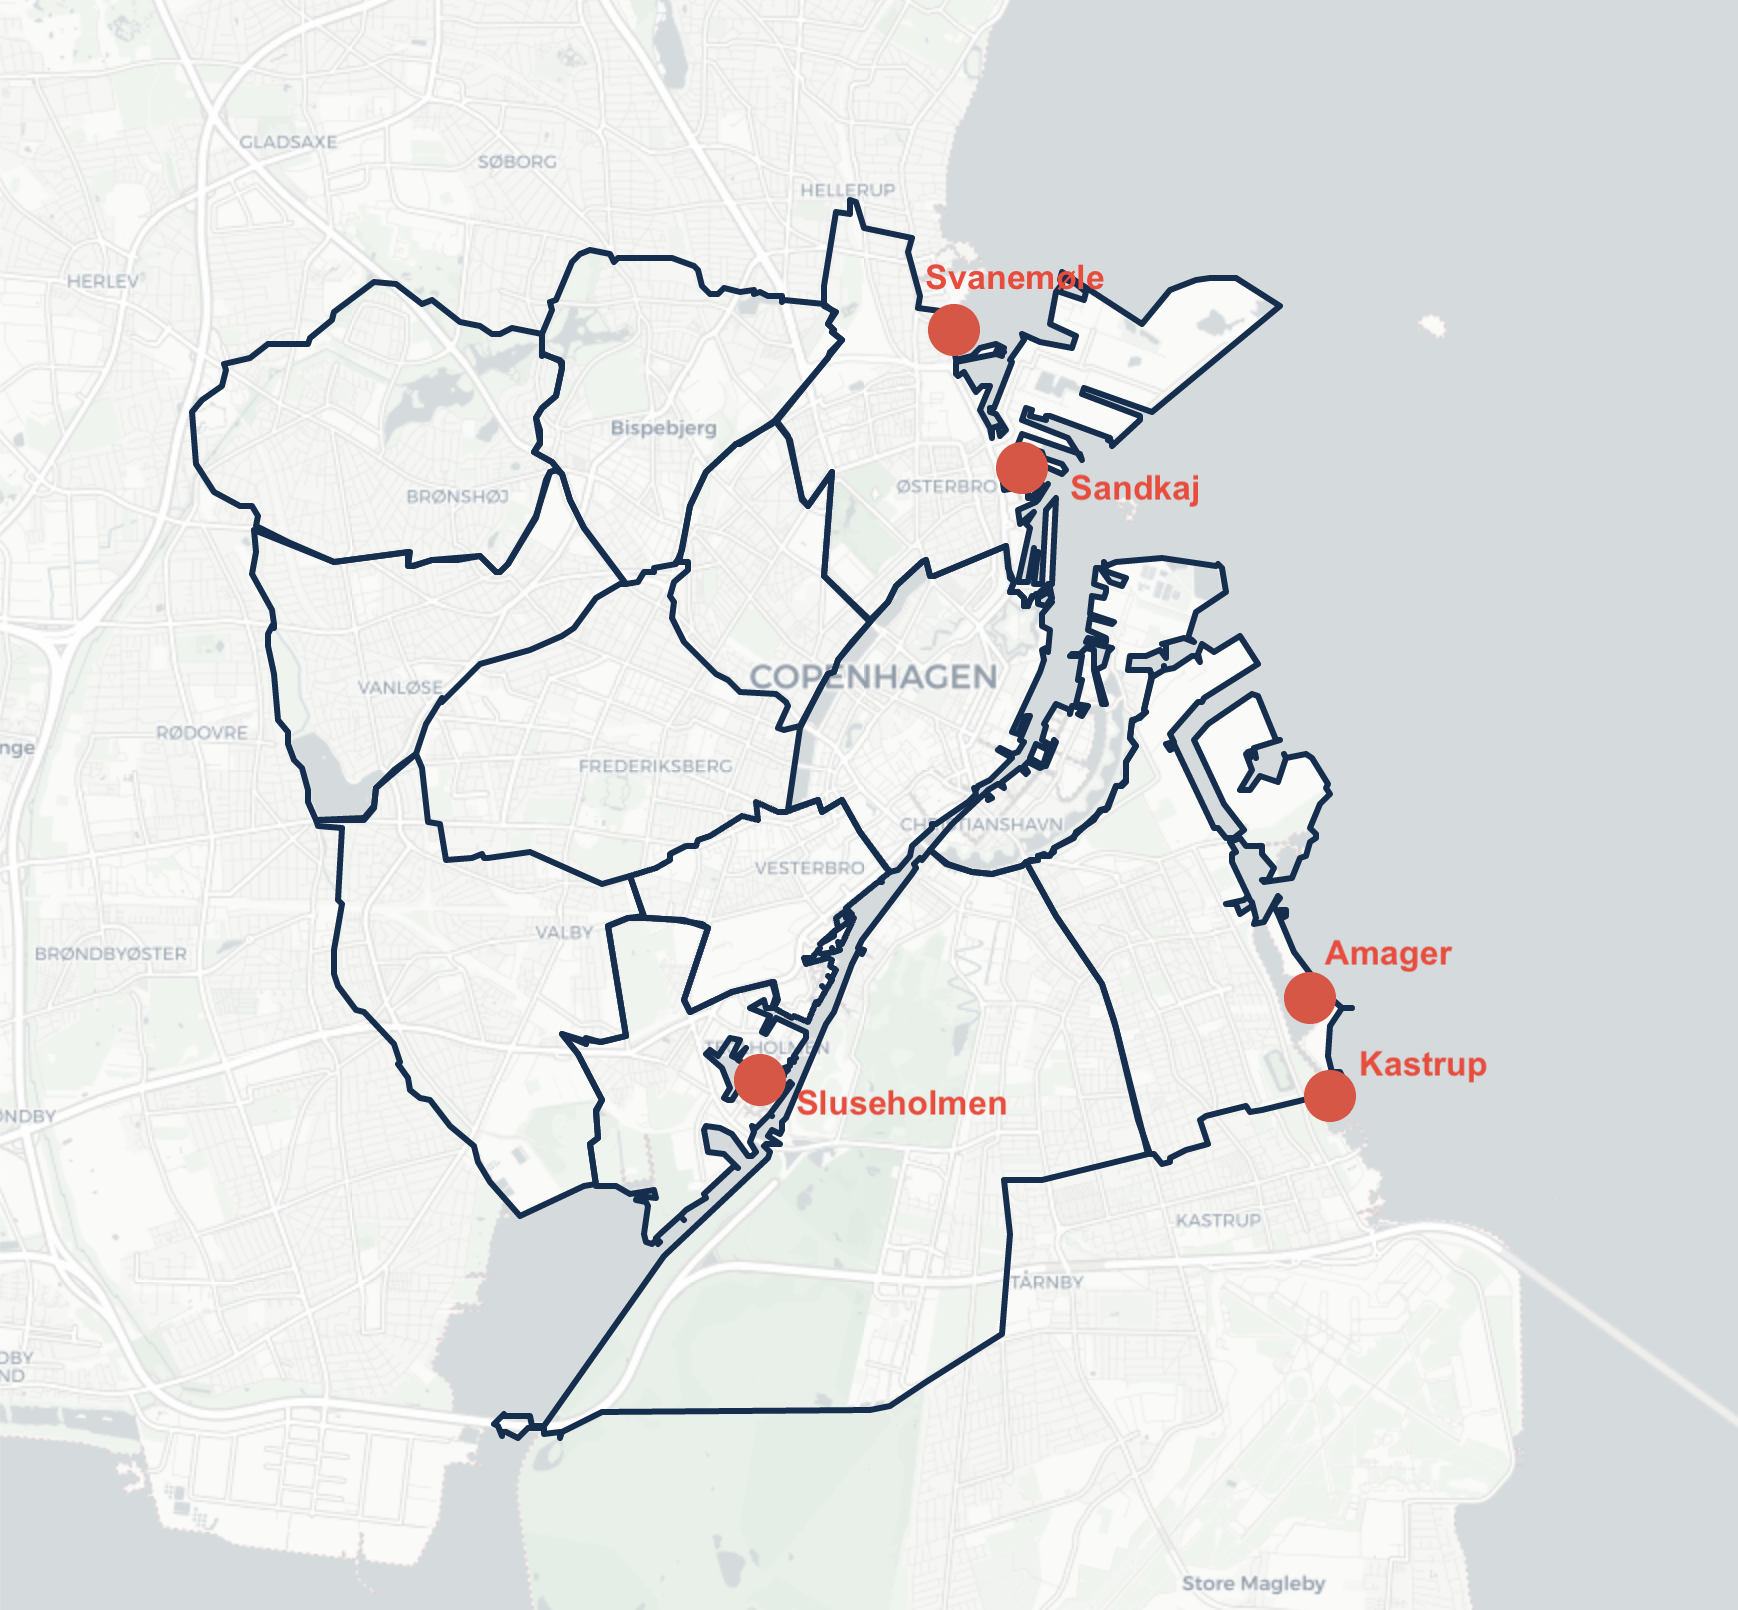
\includegraphics[width=0.8\textwidth]{copenhagen_bs_shortlist.png}
	\caption{\textit{A map of Copenhagen with the shortlisted blue spaces (in red) in their respective}}
	  \label{fig:ubs}
\end{figure}

\bisection{Sandkaj Harbour Bath} is open for swimming year-round. It is located in the Nordhavn neighbourhood of the Østerbro district, which is referred to as ``the newer part of town’’, a new and exciting area where cafes and restaurants keep opening and create a buzzing feel around the bathing zone” \parencite{visitcopenhagen_baths}.

\bisection{Svanemøle Strand} is also located in the Østerbro district north of the Sandkaj harbour, the Svanemøle beach opened in 2010. It has sand, a pier, and a promenade. Swimming can take place year-round.

\bisection{Sluseholmen Harbour Bath} is the latest harbour bath to open in 2012. It is a “protective lagoon”\parencite{visitcopenhagen_baths} with four different pools for children, youth, exercising and diving. It is supposedly used mainly by families living in the quiet and new neighbourhood \parencite{bak_2015}, due to it being out of reach compared to popular baths in the centre. This site is interesting because so far, it is intended for the local community and is not (yet?) attracting a wider crowd. Plus, both the neighbourhood and baths are new. This makes it a good location to understand how people are shaping the area, as it develops.

\bisection{Amager Beach} is a sandy beach and also has grassy lawns. It is allowed to barbecue, there are sports facilities, and many waterfront activities like volleyball, kite-surfing and snorkeling. There is a bathhouse open year-round with a wooden deck on one end of the beach.

\bisection{Kastrup Sea Bath} is just south of Amager beach, with views of Saltholm Island and Sweden, equipped with an award-winning architectural structure. It is equipped with changing rooms, showers, lockers, swimming facilities, and people can dive from the structure. The water around the structure is deep and thus not ideal for children or those uncomfortable in deep water.

%%%%%%%%%%%%%%%%%%%%
\subsection{Data collection}
%%%%%%%%%%%%%%%%%%%%

\begin{comment}
The research has the following objectives:
\begin{enumerate}
	\item To understand people's motivations for visiting, or not visiting, a particular UBS
	\item To compare a set of UBS in the city, in terms of the motivations discovered above
	\item To discuss how this knowledge can be used by city planners, to provide UBS that can be used by everyone
\end{enumerate}
\end{comment}

The data collection methods will be a combination of interviews with users of the UBS, and observations of the UBS. See Appendix A for detailed interview and observation protocols.

\subsubsection{Interviews}

Interviews with UBS users consist of structured, open-ended questions, and are estimated to take a maximum of 30 minutes to complete. The aim of these interviews is to ask users specific questions about the way they use UBS, their reasons for visiting a particular UBS, their perceptions of the physical environment and social settings, what issues may prevent them from using UBS, and what benefits they perceive UBS to provide.

Limiting the interviews to 30 minutes will allow me to collect a maximum of responses compared to more lengthy ones. And compared to surveys, a qualitative interview approach will enable me to explore in depth the motivations behind people's perceptions of the space \parencite{noel2021social}.

I aim to collect a minimum of 15 interviews per UBS, so a total of 45 across the 3 sites.

\subsubsection{Observations}

Interviews will be combined with direct observations of human activity, signs of human activity, and characteristics of the site. Previous research have identified observable factors that inhibit use of urban green space, like lack of infrastructure or the appearance of the surroundings \parencite{raymond2016integrating}, or infrastructure that attracts specific user groups (eg. sports equipment), or broken glass and vandalism \parencite{noel2021social}.

Observations of human activity will collect information on the type of activities people are carrying out, such as swimming, playing sports, walking, sitting, socialising, and so on. I will pay particular attention to the sociability of people (whether they are on their own, in pairs or groups), noise levels from people and activities, demographics (age and sex), conflicting uses and user groups.

The signs of human activity are similar, but for activities that are not happening at the time of the observation either because they happen more slowly over time, or at a different time of day or week. For example, advertised events or community groups, or signs of care or neglect.

UBS characteristics are anything in the planned environment that could influence attractiveness.
For example, the built environment (eg. paths, benches, bins), services (eg. toilets, changing rooms, lifeguards), the quality of the water (eg. pollution levels), or the surroundings (eg. nature, shops and restaurants).

Altogether, these observations express relatively objective characteristics of the UBS that feed into people's social interpretation of the space, ultimately determining whether or not they use it.

%%%%%%%%%%%%%%%%%%%%
\subsection{Data analysis}
%%%%%%%%%%%%%%%%%%%%

%Quantitative data from the observations and closed-answer responses will be entered into a spread sheet for statistical analysis. Pivot tables are a popular way to organise data to make it easier to find patterns.
% Statistical analysis ??
% Spatial analysis ??
Field observations will be entered into a spread sheet for statistical analysis.
Qualitative interview responses will be encoded. The coding scheme will be updated after each day of data collection, and serve to identify key concepts. When the encoding is complete, clustering may be applied to the codes, as recommended by Miles and Huberman \parencite{miles1994qualitative}.

After the data has been organised ,encoded and analysed, I will do a comparative analysis across the 3 UBS. Here, I might consider other UBS mentioned by users during the interviews.
Where possitble, the results will be organised spatially to convey how perceptions vary across the UBSs.

%The results from the analysis will be highly subjective, since that is the nature of perceptions. Therefore, I will not be producing an exhaustive representation of people's experiences of UBS across Copenhagen, but rather a more holistic discussion based on access and justice.

\section{Timeline and feasibility}

Many more people spend time at the water in summer compared to than winter. Therefore, I aim to collect my data starting in August and going up to October (circa 10 weeks). This should allow me to capture a wide range of users and uses. Even though swimming culture is big in Denmark and people do use UBS all year, winter swimmers are a very particular group of people compared to the more general population I plan to study.
With an estimated total of 45 interviews, I should collect an average of 5 interviews/per week, or 1-2 per UBS.

\begin{figure}[!h]
\begin{adjustwidth}{-3cm}{}
\begin{ganttchart}[
hgrid,
vgrid,
expand chart=1.3\textwidth,
time slot format=isodate-yearmonth,
time slot unit=month
]{2022-03}{2023-06}
\gantttitlecalendar{year, month} \\
\ganttbar{Thesis proposal}{2022-03}{2022-06} \\
\ganttbar{Design observation guide}{2022-07}{2022-07} \\
\ganttbar{Design interview}{2022-07}{2022-07} \\
\ganttbar{Pilot observations \& interviews (Munich, DE)}{2022-07}{2022-07} \\
\ganttbar{1st visit to UBS}{2022-08-01}{2022-08-31} \\
\ganttbar{Pilot observations \& surveys}{2022-08-01}{2022-08-31} \\
\ganttbar{Data collection}{2022-08}{2022-10} \\
\ganttbar{Literature review}{2022-09}{2022-11} \\
\ganttbar{Data analysis}{2022-12}{2023-03} \\
\ganttbar{Writing report}{2023-03}{2023-06} \\
\ganttmilestone{Thesis defence}{2023-06}
\end{ganttchart}
\end{adjustwidth}
\caption{Timeline for the research}
\end{figure}


\printbibliography

\appendix

\pagebreak
\section{Appendix A: Data Collection Protocols}

\subsection{Interview Protocol}

\begin{table}[!ht]
	\begin{adjustwidth}{-3cm}{}
    \begin{tabularx}{1.4\textwidth} { 
  | >{\raggedright\arraybackslash}X 
  | >{\raggedright\arraybackslash}X | }
    %{|l|l|}
    \hline
	Location: & Date: \\ \hline
	Time of day: & Time of week \& year:  \\ [0.5ex] \hline\hline
	\textbf{Questions} & \textbf{Link to research}  \\ [0.5ex] \hline\hline
	\multicolumn{2}{|l|}{\textit{\textbf{Background information}}} \\ [0.5ex] \hline
	1. Approximate age ($<30, <65, 65+$) - not to be asked & Demographic data \\ \hline
	2. What neighbourhood do you live in? & Demographic data; (Barriers to) availability, accessibility \\ \hline
	\multicolumn{2}{|l|}{\textit{\textbf{Use \& preference in UBS}}} \\ [0.5ex] \hline
	3. What are you doing here today, or what do you usually like to do? & Use (activity)  \\ \hline
    4. When do you come here, how often? & Use (frequency)  \\ \hline
	5. Why do you choose to come to this place? & Attractiveness \\ \hline
	6. Are there any issues that make you avoid visiting this place at any point? & Accessibility, attractiveness (barriers) \\ \hline
	\multicolumn{2}{|l|}{\textit{\textbf{Physical and social perceptions of the UBS}}} \\ [0.5ex] \hline
	7. How attractive do you find this place, why? & Attractiveness (social \& physical barriers/enablers) \\ \hline
	8. How adequate do you find the equipment or services here? & Attractiveness (physical barriers/enablers) \\ \hline
	9. How safe do you feel here? & Attractiveness (social \& physical barriers/enablers) \\ \hline
	10. How do you find the people here? & Attractiveness (social barriers/enablers) \\ \hline
	11. Do you share the same interests or experiences as people here? & Attractiveness (social barriers/enablers, belonging) \\ \hline
	12. How much can you be yourself here? & Attractiveness (social barriers/enablers, belonging) \\ \hline
	\multicolumn{2}{|l|}{\textit{\textbf{Using other UBS}}} \\ [0.5ex] \hline
	13. What other other places you like to go that are close to the water? & Availability, accessibility, attractiveness (barriers/enablers) \\ \hline
	14. Why do you (or if there are no other places - don't you) like to go to there? & Availability, accessibility, attractiveness (barriers/enablers) \\ \hline
	\multicolumn{2}{|l|}{\textit{\textbf{Perceived benefits of UBS}}} \\ [0.5ex] \hline
	15. Do you think these types of places near the water are important? Why, or why not? & Perceived benefits \\ \hline
    \end{tabularx}
	\end{adjustwidth}
\end{table} 

\pagebreak
\subsection{Observation Protocol}

\begin{table}[!ht]
	\begin{adjustwidth}{-3cm}{}
    \begin{tabularx}{1.4\textwidth} { 
  | >{\raggedright\arraybackslash} X
  | >{\raggedright\arraybackslash} X 
  | >{\raggedright\arraybackslash}p{5cm} | }
    \hline
        Location: & Date: & ~ \\ \hline
        Time of day: & Time of week \& year: & ~ \\ \hline \hline
        \textbf{Direct Observations} & \textbf{Categories/Examples} & \textbf{Link to research} \\ \hline \hline
        	\multicolumn{3}{|l|}{\textit{\textbf{Human \& social activity}}} \\ [0.5ex] \hline
	 	Age & Kids/teens ($<18$), young adults ($<35$), adults ($<65$), seniors ($65+$) & Demographic data \\ \hline
        Sex & Male, female & Demographic data \\ \hline
        Activities & \textbf{Water activities} (swimming, boating, fishing); \textbf{physical activities} (swimming, jogging, cycling, other sports, walking); \textbf{socialising} (talking, eating/drinking, party); \textbf{passive activities} (photography, drawing, reading, resting); \textbf{antisocial/illicit}; \textbf{stewardship}; \textbf{other} (homeless person sleeping, busking) & Social setting (uses) \\ \hline
        Sociability & Individuals, pairs, family, small groups ($<10$), large groups ($10+$) & Social setting (uses) \\ \hline
        Crowdedness of the place & Measure by density? & Social setting\\ \hline
        Noise levels & ~ & Social setting \\ \hline
        Encounters & Positive/negative encounters between people; conflicts between activities/groups; policing & Social setting \\ \hline
        \multicolumn{3}{|l|}{\textit{\textbf{Traces of human \& social activity}}} \\ [0.5ex] \hline
        Advertised events & Community board; posters & ~ \\ \hline
        Signs activities & Signs of any activities listed above (equipment, advertisements) & ~ \\ \hline
        Signs of care or neglect & Stewardship, art; trash, vandalism & ~ \\ \hline
		\multicolumn{3}{|l|}{\textit{\textbf{Characteristics of the site}}} \\ [0.5ex] \hline
		Built environment & Places to sit, tables, accessibility of paths, bins & Physical environment \\ \hline
        Services & Toilets, changing rooms, lifeguards & ~ \\ \hline
        Quality of the water & Pollution, trash & Physical environment \\ \hline
        Scenery & Wild vs. curated nature, diversity of the nature & Physical environment \\ \hline

	\end{tabularx}
	\end{adjustwidth}
\end{table} 

\end{document}

%%%%%%%%%%%%%%%%%%%%%%%%%%%%%%%%%%%%
%				COMMENTS
%%%%%%%%%%%%%%%%%%%%%%%%%%%%%%%%%%%%

\begin{comment}
THESIS NOTES

Limitations:
- Observations done by a single person may not be reliable, would be more reliable and richer if conducted by 2 researchers who could debrief their observations and discuss their interpretations; Plus, how objective can observations be? 
- Only interviewed users, and not non-users of UBS
\end{comment}
